\documentclass[11pt]{article}
% Packages used by instructor %
\usepackage{amsmath,amssymb,xspace,epsfig}

% Package used for setting up page margins %
\usepackage{geometry}
%\usepackage{showframe} % Used to clearly show the new margins %
\newgeometry{vmargin={1in}, hmargin={1in,1in}}

% Package used for adding hyperlinks %
\usepackage{hyperref}
\usepackage[anythingbreaks]{breakurl}

% Package for multirow tables %
\usepackage{multirow}
\renewcommand{\arraystretch}{1.5}

% Package for Bib in ToC %
\usepackage[nottoc]{tocbibind}

\usepackage{subcaption}
\usepackage{wrapfig}

% Page Header %
\usepackage{fancyhdr}
\pagestyle{fancy}
\fancyhf{}
\lhead{Natural Language Processing\\ Home Work 4}
\rhead{Narayan Acharya \\ 112734365}
\lfoot{}
\rfoot{\thepage}

\renewcommand{\headrulewidth}{1pt}
\renewcommand{\footrulewidth}{1pt}

\title{
	Natural Language Processing - Home Work 4\\[2mm]
	\large CSE 538 Fall '19\\[1mm]
	\textit{Prof. Niranjan Balasubramaniam}
}
\author{
	\small Submission By: \\
	\href{mailto:nacharya@cs.stonybrook.edu}{Narayan Acharya} \\
	\small 112734365
}
\date{\vspace{-5ex}}
\begin{document}
	
% Set up title
\maketitle
\thispagestyle{fancy} % Make this page use fancy header

% Set up Table of Contents
\tableofcontents

\section{Base Model: GRU Implementation}
\begin{enumerate}

\item \textbf{Model Architecture:} 

Our model is a neural network for relationship extraction. We try to emulate the model as mentioned in the paper \cite{GRUBaseModel}. In accordance with the model architecture in the paper we build a 3 layer architecture - Bi-directional GRU layer, an attention layer, and an output layer. [The architecture in the paper has an additional embedding layer mentioned separately as well.]

For the first layer, we have a Bi-directional GRU. The input to the GRU is a concatenated tensor for our word embeddings and Part of Speecg (PoS) embeddings. The shape of the input to this layer is [$batch\_size$, $sequence\_length$, $embeddings\_size$]. In our case, we used GloVe embeddings of 100 dimension for both words and PoS. Therefore on concatenating we received a 200 dimensional embedding for every token in our input, i.e. $embeddings\_size$ is 200. $sequence\_length$ is the maximum number of token in the current batch. For sequences with lesser than the max number of tokens, we have padding (zeros) appended to the input. In order to work with this, we use a mask along with our input to the GRU to indicate to the GRU of what values it needs to be working on and which ones to ignore.

The second layer is our attention layer. We calculate the attention based on the equations 9, 10, 11 and 12 as suggested in the paper \cite{GRUBaseModel}. The input to the attention layer is the output from the GRU layer of shape [$batch\_size$, $sequence\_length$, $2 \times hidden\_size $]. The output of the attention layer is a tensor of shape [$batch\_size$, $2 \times hidden\_size$] which is essentially a sentence representation for each sentence in our batch. The important deviation from the equation is our calculation of $ r $ in equation 11 from the paper is where in the calculation of $H\alpha^T$ we take a weighted sum of the output vectors, something not clearly mentioned as part of the equations but is mentioned in the text.

The final layer, is the output layer which takes in the output of the attention layer and outputs a tensor of shape [$batch\_size$, $num\_classes$]. This is essentially a fully connected/dense layer that acts as our classification layer to assign probability of the input in each of the possible 19 classes. We have 9 possible relationship classes, but since they can be different in each direction, we get 18 different possibilities from them and we have one class which we use the 'Other' class.

Another task was to calculate the regularization loss, using a regularization factor of $ 10^{-5} $, as mentioned in the paper while back-propagating the gradients back through our network. The regularization loss consists of L2 loss for all our trainable variables in the model.

\item \textbf{Observations of experiments:}

As part of the base model, we look to carry out certain experiments as outlines in table \ref{tab:experiments-gru}.

\begin{table}[]
	\centering
	\begin{tabular}{|c|c|}
		\hline
		\textbf{Experiment} & \textbf{\begin{tabular}[c]{@{}c@{}}F1 Score\\ (5 epochs)\end{tabular}} \\ \hline
		Baseline - Word + PoS + Shortest Path & \textbf{0.5683} \\ \hline
		Experiment 1 - Only Word Embeddings & 0.5503 \\ \hline
		Experiment 2 - Only Word + PoS Embeddings & 0.5115 \\ \hline
		Experiment 3 - Only Word + Shortest Path & 0.5886 \\ \hline
	\end{tabular}
	\caption{Bi-GRU Experiments Comparison}
	\label{tab:experiments-gru}
\end{table}


Some inferences one can draw from the results of the experiments:
\begin{enumerate}

	\item From the results for the baseline and experiment 3, one can infer that calculating the shortest path is critical for better performance. The shortest path possibly focuses our model to only use the most important/relevant information for the task at hand.
	
	\item Using just the word embeddings, like in experiment 1, is not sufficient information for our model to confidently classify the relationship into the possible classes.
	
	\item Extra information, like that of the PoS tags, like in experiment 2, without the shortest path did not help but actually decreased the F1 score. We gave our model too much information for it to reliably choose from the possible classes. The PoS tags of only the words around our entities seem to have a say in the class of the relation rather than all the tokens in the entire context.
		
\end{enumerate}

\end{enumerate}
\section{Advanced Model: CNN with Multiple Filter Convolution \& Max Pooling}

\begin{enumerate}
\item Model Inputs:
The advanced model I chose was loosely based on the paper \cite{CNN}.
The model performed better than the baseline GRU model and uses only word embeddings and positional embeddings(as defined below) for the task. PoS embeddings and shortest path were \textit{not} used.

Positional Embeddings: We assign numerical values to tokens based on how close to our entities they are. Consider the following example:

\begin{center}
	\textit{The \textbf{ship} is in the \textbf{dock}.}
\end{center}

\textbf{ship} and \textbf{dock} here are our two entities and lets say the relation between the two is \textit{Contains(\textbf{dock}, \textbf{ship})}. We assign positional embeddings based on both entity 1 and 2, which will look something like this for our case as shown below.

\begin{equation*}
position\_1 = [1, 0, 1, 2, 3, 4]
\end{equation*}
\begin{equation*}
position\_2 = [5, 4, 3, 2, 1, 0]
\end{equation*}

Notice that entities are at positions 1 and 5 (indexing based on 0) in our sentence, where $ position\_1 $ and $ position\_2 $ mark them as 0 and as you move away from them, the positional values increases by 1.

\item Model Architecture:

High level architecture of the advanced model can be seen in figure \ref{fig:advanced-model}
\begin{figure}[!ht]
	\centering
	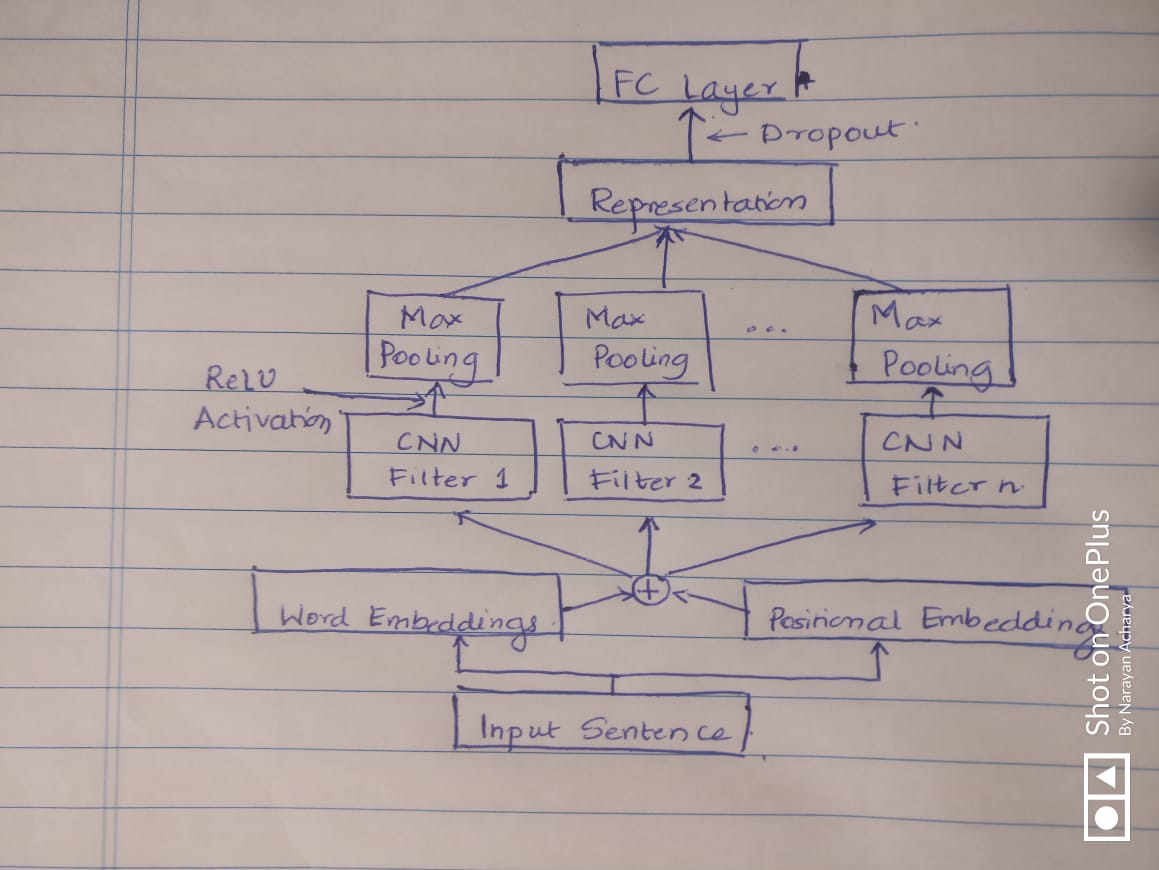
\includegraphics[width=0.8\textwidth]{advanced-model.jpeg}
	\caption{Advanced Model: High Level Architecture}
	\label{fig:advanced-model}
\end{figure}

We perform similar steps to tokenize our sentence like we did in the base model and get the word token, which we then use our GloVe embeddings for finding the representation of the word. We also calculation position values as shown above. We also maintain an embedding matrix for these positional values, which we learn as we train our model. We then concatenate the word embedding, position according to entity 1 embedding and position according to entity 2 and use this as our input to the next layer.

In the next layer, we convolve filters of multiple sizes across the input from the previous layers, the embeddings in this case. We use ReLU activation with each CNN filter and use Max Pooling on top of each.

After each of the filters are applied, we concatenate the output from each into a single representation and flatten it out to pass to our Fully Connected Layer for acting as the final classification layer. We use dropout before we send it to Fully Connected layer to address for over-fitting.

NOTE: For position embeddings, another approach one can try out (not done as part of this assignment) is assigning higher numbers to the entities that decrease as you move from the entity token indices. This intuitively fits better with how we convolve and use Max-Pooling on the the convolved outputs.

\item Model Parameters \& Performance:

We use the following parameters for training our model which varies slightly from the numbers as suggested in the paper.

\begin{enumerate}
\item We use GloVe embeddings of dimension 300. We define the positional embeddings to be of size 100. GloVe embeddings are \textit{not} pre-trained while positional embeddings are something we learn as we train.

\item We use 4 filter sizes of value 2, 3, 4, 5 and each filter size having 128 filters. We use ReLU activation and Max-Pooling with each filter size.

\item We use a dropout value of 0.3 and a mini-batch size 0f 20 for training across 6 epochs.
\end{enumerate}

With the above parameters the model got an F1-score of 0.6289 which is better than the baseline Bi-GRU model which got an F1 score of 0.5683 with word, PoS and shortest path features.

Other experiments were run as:
\begin{enumerate}
\item Tweaking the batch size to 30 and training for 5 epochs resulted in an F1 score of 0.6191.
\item Tweaking the embedding dimension used to be 200 over training 5 epochs resulted in an F1 score of 0.58.
\end{enumerate}

\end{enumerate}

\bibliographystyle{unsrt}
\begin{thebibliography}{9}
	\bibitem{GRUBaseModel}
	Attention-Based Bidirectional Long Short-Term Memory Networks for
	Relation Classification,
	\\\texttt{\burl{https://www.aclweb.org/anthology/P16-2034.pdf}}
	\bibitem{CNN}
	Relation Extraction: Perspective from Convolutional Neural Networks,
	\\\texttt{\burl{https://cs.nyu.edu/~thien/pubs/vector15.pdf}}
\end{thebibliography}
	
\end{document}